\section{Graph observer}
\label{sec:dagObserv}
One of the main objectives of the Flatland-Challenge is to find a suitable observation (relevant features for the problem at hand) to solve the task. For this reason the Flatland library provide full flexibility when it comes to building your custom observations. Whenever an environment needs to compute new observations for each agent, it queries an object derived from the \textit{ObservationBuilder} base class, which takes the current state of the environment and returns the desired observation.\\
We had at our disposal for testing the environment many observer:
\begin{itemize}
\item TreeObsForRailEnv
\item GlobalObsForRailEnv
\item LocalObsForRailEnv
\end{itemize}
Anyway for our comprehension of the environment these default version could not be able to perform at best with a RL approach since they compute a view of the environment focused on unnecessary details and more importantly they describe just the agent neigbourhood without giving contextual information to the external \textit{entity} which has to choose the action to perform. Some of them were considered for a deeper analysis and testing but as we have hypotesized the performance were not good.\\
We opted for a custom observation based on a graph inspired by the TreeObserver but with a totally different structure. In particular what we requested from the observer entity was:
\begin{itemize}
    \item ease the search path as much as possible since the management of transitions and direction feasibility can be quite a complex job in bigger environments.
    \item be able to retrieve the recurrent information for a certain point in the space in linear or at maximum in polynomial time.
    \item reduce the search space and decrease the search time for the identification process of the shortest path at each step of the agents, but still maintaining a good level of explainability in the resulting view.
    \item build an observation with data and structures properly formatted with the aim of feeding a network model with it and later on reduce the effort necessary for the training.
\end{itemize}

Our implementation can be found under the class \textit{DagObserver}. It extends the base class ObservationBuilder and implements the standard behaviour including the initialization of the environment variables, data structures and the reset procedure to be executed at the end of each episode. Moreover there are the \textit{get} methods (single and multi agent) which are invoked at each environmental step to obtain the observation of each agent.\\
In our implementation the reset method is also in charge of the creation of the initial \textit{general\_graph} which will be used during the entire episode to calculate the paths and foresee the movements of the agents. Furthermore particular attention has been dedicated to the the order of computation of the single observations: the \textit{get\_many} method instead of iterating over the cardinal dictionary of agents and call the \textit{get} method, uses a list of agents ranked by priority. Our intuition was inspired by common rules used while driving the car:
\begin{itemize}
    \item a slow driver self aware of their ability to give the priority to the others when in doubt
    \item a normal driver knows that in presence of some signals like the sirens of an ambulance/police he should absolutely give way
    \item a fast driver is probably more careless/irresponsible. He will surely arrive faster at the destination assuming he won't make an accident...
\end{itemize}
In the same manner we calculated an index which summarizes the characteristics of an agent and influences the level of attention that he uses to avoid conflicts with others. The more priority has an agent the less he cares about possible conflicts. Although this could seem a selfish implementation, it must be considered that the other agents, being more careful (less priority) will be able to detect and avoid the incident giving way to the opponent.\\
Then, after being computed, the observations are stored in the \textit{prev\_observations} dictionary for future uses and returned as output value to the caller, the  \textit{FlatlandRailEnv}.


\subsection{General graph}
This graph is an abstract but detailed view of the rail grid environment. It's built with the specific aim of store and rapidly retrieve information from whatever initial position or path taken on consideration for the exploration. That is of primary importance since the structure of the graph itself is a simplification of the real transition system provided by the environment and would be used during each step search process. That indeed requires to have an optimal time of access for certain information being accessed frequently. Some of them are also encoded in the structure of the graph, for instance the orientations and access point associated to the nodes which dictate the possibilities of movement of an agent during a traverse process.
\begin{figure}[H] 
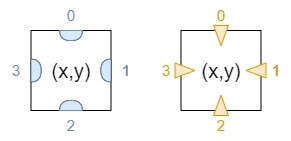
\includegraphics[scale=0.8]{figures/orientations.jpg}
\centering
\caption{Rail orientations}
\end{figure}
\noindent
For each pair of switches directly linked in the rail there is a connection in the graph too.\\
The main point in favour of such a structure is that it results in a reduced space of the real environment and it can be used with ease for the process of path discovery from source to target. De-structuring the rail environment we can indeed extract possible valuable paths which will be verified in a second moment controlling the feasibility of each transition from node to node.\\
A failure is encountered when, for instance, the path uses two consecutive switches between which a feasible transition that considers the orientation of the agent doesn't exist. Note that, it is not necessarily a bad event since the observation algorithm is able to explore the graph resuming from the failure node reached, and can then calculate a new shortest path to the target. Moreover the invalid transition is saved and will be taken in consideration during the future path discovery processes. \\
The graph also registers events of deadlocks or starvation situations: updating the status of the environment with those events can be handled properly thus minimizing the probability of future problems.\\
At each step of an episode that process is replicated for each agent to improve the structure reliability of the \textit{general\_graph} and at the same time the current observation from the agent position is built. Most of the changes to the initial graph are not permanent since it will be resetted at the end of each agent step allowing different paths discovery in the successive situations. That has been evaluated as a good compromise between state management retainment and the computational cost of evaluating each time the environment, due to its dynamicity.

\subsubsection{Deadlocks and starvations}
The general graph allow also to spot edge cases in which the target is unreachable:
\begin{itemize}
    \item Deadlock: detected when from the start point of the agent another agent incoming in the opposite direction is found before a switch cell.
    \item Starvation: happen when the procedure of minimum path search is unable to return a value 
\end{itemize}
In case of a deadlock the agents are forced to move until they are stuck one in front of the other with no more possibility of action. This is motivated by the handling of the starving agents. We thought that in cases where the target reachability is negated for an agent but he still can move, his presence can be harmful to other agents therefore he will be marked as "starving" and sent to "die" in a deadlock edge position. Compacting the agents in with deadlock status into an edge allow to have more space for other agents in such a dead rail.\\
The only situation that will cause a permanent resize of the graph is a deadlock event with the parameters \textit{steps\_to\_deadlock} to 0 and \textit{first\_time\_detection} True. That happens when the agent is stuck with another agent (no possibility of going forward) and the decision of entering in such a rail, with the consequent deadlock detection, has just been made (hence the previous cell is a switch). To handle that situation the edge in the same direction as the agent is removed and recursively the transitions of the nodes involved are controlled, eventually deleting also the descendant edges if such node hasn't a valid transition in the specific orientation anymore.\\\noindent
The deadlock event can also happen on a switch: in such case all the rails going toward that switch are removed.

\subsubsection{Structure}
The structure of the graph can be seen from the following image showing the rail and the corresponding graph representation:
\begin{figure}[H] 
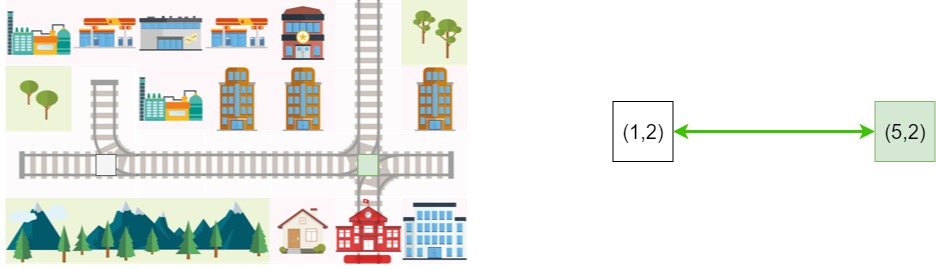
\includegraphics[scale=0.45]{figures/general-graph.jpg}
\centering
\caption{General graph}
\end{figure}
For each switch there is a node with associated a pair of coordinates (x,y) while each edge represent a rail between the switches. It can be observed that two switches could be connected by more than one rail depending on the access point used for the transition. To handle that requirement, the graph data structure has been implemented with a \textit{MultiDiGraph}.\\
The nodes contain information relative to:
\begin{itemize}
    \item Transitions: a matrix 4 by 4 of zeros or ones.
    \item Node transitions: a matrix 4 by 4 where the values are the nodes reachable with a transitions from a certain orientation and access point.
    \item Dead end: the presence of dead ends which can be used to return to the same switch, specified with access point to use and cost associated.
    \item Targets: the presence of targets in a certain direction from the current node.
\end{itemize}
The edges contain information about:
\begin{itemize}
    \item Weight: the steps between the two nodes.
    \item Access point: specify which access point will be used for both ends of the edge. It's useful since the exit direction wrt the edge direction is also the key identifier of the edge itself.
\end{itemize}

\subsection{Direct acyclic graph}
The expressivity of that graph is much higher but its existence is retained to the observation of the single agent in the current environment situation. It lacks all of the navigation information that can instead be found in the general graph, since its main focus is to represent explicitly a path from a start point to the target driving the decision of the model for the next action selection for the agent. The construction process aims to find the best (shortest) path from the agent position to one of the possible switch positions that give access to the target, moreover we implemented a behaviour aimed at exploring other possible paths and also possible interactions with other agents.\\
In detail the first search of a path is executed scanning the initial graph without the other agents, then a second search is made removing the edges in use by the other agents but in the opposite direction, in a way to find a path which avoids them. The final step is about marking the nodes with the \textit{conflict} label if they appear at a certain distance from the start node both in the current agent observation and in the observation of another agent with higher priority.
The idea as explained before is that who has a lower priority should take care of possible conflicts with who has an higher priority.

\subsubsection{Structure}
The structure of the graph can be seen from the following image showing the translation from the the general graph for the agent represented:

\begin{figure}[H]
\begin{adjustwidth}{-1cm}{}
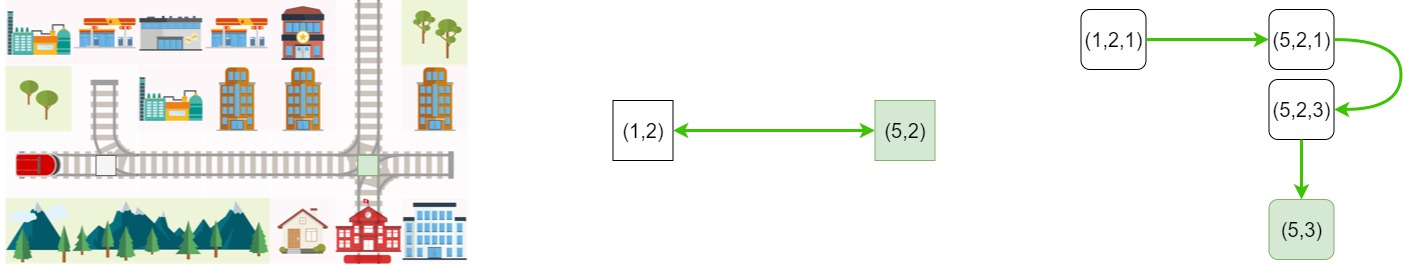
\includegraphics[scale=0.35]{figures/direct-graph.jpg}
\caption{Direct graph}
\end{adjustwidth}
\end{figure}
Each node is represented with a triple of coordinates and orientation (x,y,dir), therefore each switch is represented uniquely considering the direction of access. The graph/rail correspondence is valid for all the nodes except for the target position which is represented with a tuple of coordinates being not a switch cell. The starting node is instead approximated to the nearest switch which involves a decision for the agent.\\\noindent
Note that given the construction procedure used, the graph can also be commonly considered as acyclic.\\
\noindent
The following are the labels and the piece of information stored in the graph. Their primary role is to enable statistics computation and allow the identification of the precise role of a node in the graph, giving a reference structure for the model learning process.
\begin{itemize}
    \item \textit{START}: represent the start node and contains the information of the current agent like "velocity", "switch\_distance", "nr\_malfunctions", "next\_malfunctions", "malfunction\_rate", "malfunction".
    \item \textit{TARGET}: assigned to the target node.
    \item \textit{DEADLOCK}: it indicates that the agent is in an unrecoverable situation. Additional info provided are "steps\_to\_deadlock" and "first\_time\_detection".
    \item \textit{CONFLICT}: the choice of that node can give rise to a deadlock situation with another agent. The following information describe the characteristics of the opponent: "velocity", "conflict\_distance", "target\_distance", "nr\_malfunctions", "next\_malfunctions", "malfunction\_rate", "malfunction".
    \item \textit{STARVATION}: that label can be found in the start node in case it doesn't exist a path for the agent to reach it's target.
    \item \textit{DEAD\_END}: nodes that can be reached with the exploit of a dead end in the previous step.
\end{itemize}


\subsection{\textit{get} procedure}
The \textit{get} procedure is the main call of the observer and is in charge of computing and returning the observation for an agent.
The method can be summarized in the following points:
\begin{itemize}
    \item The directed graph is created and the general graph structure and data are copied in a new object so the subsequent modifications won't affect the original structure.
    \item From the position of the agent the path is scanned until a switch cell which need a decision from the agent. In that rail portion possible combinations of events are handled and the first switch position is then added as starting node. In case of a deadlock the start node is labelled properly and the process return the graph as it is, instead when target is encountered or the number of steps performed to reach the switch is greater than 1 a None object is returned since no action is required.
    \item In the remaining cases (before a switch or over it) the target is computed and added to the graph already linked to the \textit{ending\_points}: the switches from which is possible to reach the target position or the deadlock positions in case of a starving agent.
    \item The first step of path search is forwarded on the general graph without the other agents. In the method \textit{\_build\_paths\_in\_directed\_graph} the search process extracts a sequence of nodes as a valid shortest path and that is then checked evaluating the validity of the transitions between the nodes. This process proceeds in parallel with the creation of the direct graph which is compiled with only the decision switches found in the path. In case of a rejection of a sequence of nodes for missing or invalid transition the two nodes and current orientation are saved and that denied rail will be considered in the next search iterations. The path followed till the negated node is maintained as valid, and a new iteration is forwarded with ever the same targets (the \textit{ending\_points}) but with the node found to be unreachable as start position: if the path in which it was included was optimal, but invalid, probably there could be a slight deviation which makes it valid and also optimal in cost value.\\
    The search is repeated until all the nodes of an extracted path are in the directed graph and they are all connected sequentially.\\ 
    Note that in case of a failure in the path detection process, the observation graph is labelled with the starvation flag. The \textit{ending\_points} are replaced with deadlock positions and the search is reiterated.\\
    \item The second step is forwarded as previously but this time the general graph has been updated removing all the edges which will take to face another active agent. The edge removing process is iterative and therefore all the resulting unusable nodes are removed.
    \item The third and last step is in charge to label the conflict nodes. There we make use of the previous cited ranking by priority of the agents. Since the computation of the observations happens by priority order, we have at our disposal all the observations of agents with higher priority. Consequently we can match the nodes in the graphs, just by x and y, to find common nodes and therefore possible conflicts in a certain range from the start node.
    \item The resulting observation can then be returned to the train cycle
\end{itemize}
\vspace{1cm} 
It can be observed that this implementation separates the actual search of the minimum path from the detection of a feasible way. Extracting a minimal path each time and trying to traverse the nodes with that trace allows us to discover other sub-optimal paths, gives more way to learn to the model, and indirectly allowing the agent to reach his target more easily and with optimal results.


